\section{Phương pháp trích xuất quan hệ}\label{sec:phuong-phap-trich-xuat-quan-he}

\subsection{Các phương pháp truyền thống}\label{subsec:cac-phuong-phap-truyen-thong}

\begin{singlespace}
    Như được thể hiện trong Hình 1,
    các phương pháp trích xuất quan hệ (RE) hiện có có thể được phân loại thành hai loại chính:
    Phương pháp truyền thống (\underline{Traditional Methods}) và Phương pháp học sâu (\underline{Deep Learning Methods}).
    Phương pháp truyền thống sử dụng các kỹ thuật dựa trên luật (\underline{Rule Based Methods}) hoặc kỹ thuật học máy để trích xuất một tập hợp các quan hệ được xác định trước từ một kho văn bản (corpus).
    Các phương pháp truyền thống có thể được phân loại chi tiết thành phương pháp dựa trên luật (\underline{Rule Based Methods}) và phương pháp học máy (\underline{Machine Learning Methods}).
\end{singlespace}

\begin{singlespace}
    Các phương pháp học máy (\underline{Machine Learning Methods}) có thể được phân loại thêm thành bốn loại:
    (1) Phương pháp không giám sát (Unsupervised Learning Methods).
    (2) Phương pháp có giám sát (Supervised Learning Methods).
    (3) Phương pháp bán giám sát (Semi-supervised).
    và (4) Phương pháp Giám sát từ xa (Distant supervision).
\end{singlespace}

\begin{figure}[h!]
    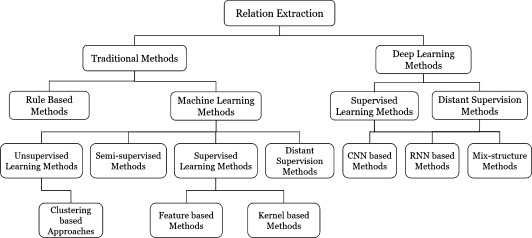
\includegraphics
    [width=0.9\textwidth]{image/parts/1}
    \begin{center}
        \begin{tablenotes}
            \item{Nguồn: https://www.sciencedirect.com/science/article/pii/S2667305323000698#br0060}
        \end{tablenotes}
    \end{center}
    \renewcommand{\figurename}{Hình.}
    \caption{Các loại phương pháp trích xuất quan hệ.}\label{fig:image/parts/1}
\end{figure}

\begin{itemize}
    \item Phương pháp dựa trên luật ({Rule-based}): Sử dụng các quy tắc thủ công được thiết lập sẵn để trích xuất quan hệ.
    \item Phương pháp không giám sát (Unsupervised): Tự động học các mẫu trích xuất quan hệ từ dữ liệu.
    \item Phương pháp có giám sát (Supervised): Sử dụng dữ liệu được dán nhãn để huấn luyện mô hình trích xuất quan hệ.
    \item Phương pháp bán giám sát (Semi-supervised): Kết hợp dữ liệu được dán nhãn và không được dán nhãn để huấn luyện mô hình.
    \item Phương pháp giám sát từ xa (Distant supervision): Sử dụng dữ liệu gián tiếp để huấn luyện mô hình.
\end{itemize}

\subsubsection{Phương pháp dựa trên luật ({Rule-based})}
Các phương pháp này còn được gọi là phương pháp mẫu thủ công (hand-built pattern methods).
Chúng xác định một tập hợp các mẫu trích xuất (\href{https://www.sciencedirect.com/topics/computer-science/extraction-pattern}{extraction patterns}) cho các quan hệ được định nghĩa trước.
Sau đó, các mẫu trích xuất này được đối chiếu với văn bản. Nếu một mẫu khớp với văn bản, thì một quan hệ tương ứng với
mẫu đó được tìm thấy trong văn bản.
\href{https://www.scopus.com/record/display.uri?eid=2-s2.0-0027709268&origin=inward&txGid=dd620e007b93bb0bb26ec41071050554}{Riloff (1993)},
\href{https://scholar.google.com/scholar_lookup?title=Fastus%3A%20A%20finite-state%20processor%20for%20information%20extraction%20from%20real-world%20text&publication_year=1993&author=D.%20Appelt&author=J.%20Hobbs&author=J.%20Bear&author=D.%20Israel&author=M.%20Tyson}{Appelt et al. (1993)},
\href{https://scholar.google.com/scholar_lookup?title=Snowball%3A%20Extracting%20relations%20from%20large%20plain-text%20collections&publication_year=2000&author=E.%20Agichtein&author=L.%20Gravano}{Agichtein và Gravano (2000)},
\href{https://scholar.google.com/scholar_lookup?title=Avatar%20information%20extraction%20system&publication_year=2006&author=T.%20Jayram&author=R.%20Krishnamurthy&author=S.%20Raghavan&author=S.%20Vaithyanathan&author=H.%20Zhu}{Jayram et al. (2006)},
\href{https://www.scopus.com/inward/record.url?eid=2-s2.0-77951560898&partnerID=10&rel=R3.0.0}{Shen et al. (2007)},
\href{https://scholar.google.com/scholar_lookup?title=RelEx%20relation%20extraction%20using%20dependency%20parse%20trees&publication_year=2006&author=K.%20Fundel&author=R.%20K%C3%BCffner&author=R.%20Zimmer}{Fundel et al. (2006)},
\href{https://scholar.google.com/scholar_lookup?title=A%20rule-based%20relation%20extraction%20system%20using%20dbpedia%20and%20syntactic%20parsing&publication_year=2013&author=K.%20Nebhi}{Nebhi (2013)} đã sử dụng các phương pháp dựa trên luật để trích xuất quan hệ từ văn bản.
Bảng 3 hiển thị các ví dụ về quy tắc để trích xuất quan hệ hạ đẳng (hyponymy) từ văn bản.


%\begin{tabularx}{\textwidth}{p{5cm}|p{5cm}|p{5cm}|}
%\hline
%Pattern & Input sentence & Extracted relations \\
%\hline
%such NP as & \ldots works by such authors as Herrick, Goldsmith, and Shakespeare.
%& Hyponym (“author”, “Herrick”),  Hyponym (“author”, “Goldsmith”),  Hyponym (“author”, “Shakespeare”)
%\hline
%NP {, NP}{,} & Bruises, wounds, broken bones or  other injuries\ldots
%& Hyponym (“bruise”, “injury”),  Hyponym (“wound”, “injury”),  Hyponym (“broken bones”, “injury”)
%\hline
%\end{tabularx}

\begin{figure}[h!]
    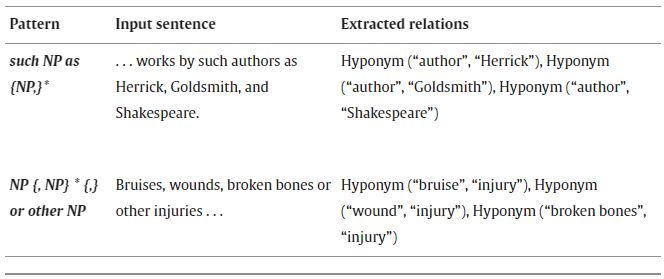
\includegraphics
    [width=0.9\textwidth]{image/parts/2}
    \begin{center}
        \begin{tablenotes}
        \end{tablenotes}
    \end{center}
    \renewcommand{\figurename}{Hình.}
    \caption{Ví dụ cho partern (mẫu/luật) Hyponyms (\href{https://www.sciencedirect.com/science/article/pii/S2667305323000698#br0500}{Hearst (1992)}).}\label{fig:image/parts/2}
\end{figure}

Các phương pháp dựa trên luật đòi hỏi chuyên môn về lĩnh vực và kiến thức ngôn ngữ để xác định các mẫu trích xuất.
Những phương pháp này phụ thuộc vào từng lĩnh vực cụ thể, trong đó cấu trúc của tài liệu là cố định và các quan hệ mục
tiêu được xác định trước. Nếu chuyển từ lĩnh vực này sang lĩnh vực khác, thì cần phải xác định lại một tập hợp mới các
quan hệ mục tiêu và mẫu trích xuất. Do đó, các phương pháp dựa trên luật đòi hỏi nhiều công sức thủ công và không thể sử
dụng cho các tập văn bản đa dạng (heterogeneous corpora).


\newpage

\subsubsection{Phương pháp không giám sát (Unsupervised)}
Phương pháp không giám sát không yêu cầu bất kỳ dữ liệu được dán nhãn nào. Hầu hết các phương pháp RE không giám sát sử
dụng cách tiếp cận dựa trên cụm (clustering). Một trong những phương pháp RE không giám sát dựa trên cụm tiên phong
được đề xuất bởi
\href{https://www.sciencedirect.com/science/article/pii/S2667305323000698#br0470}{Hasegawa et al. (2004)}. Họ sử dụng công cụ đánh nhãn Thực thể Danh riêng (NE) để trích xuất các thực
thể, cho phép tập trung chỉ vào các quan hệ với những thực thể được đề cập. Hình 2 minh họa các bước của phương pháp
học không giám sát:
\begin{itemize}
    \item (1) Nhận dạng các thực thể tên riêng trong kho văn bản.
    \item (2) Xác định các thực thể tên riêng đồng xuất hiện và ngữ cảnh của chúng.
    \item (3) Cụm các cặp thực thể dựa trên tính tương đồng ngữ cảnh.
    \item (4) Gán tên quan hệ ngữ nghĩa cho mỗi cụm.
\end{itemize}

\begin{figure}[h!]
    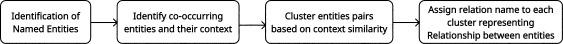
\includegraphics
    [width=0.9\textwidth]{image/parts/3}
    \begin{center}
        \begin{tablenotes}
        \end{tablenotes}
    \end{center}
    \renewcommand{\figurename}{Hình.}
    \caption{Cách tiếp cận dựa trên phân cụm cho \href{https://www.sciencedirect.com/topics/computer-science/unsupervised-learning}{Unsupervised Learning}.}\label{fig:figure2}
\end{figure}


\subsubsection{Phương pháp có giám sát (Supervised)}
Phương pháp có giám sát yêu cầu một lượng lớn dữ liệu huấn luyện được dán nhãn với tập hợp các thực thể và quan hệ. Phương pháp này sử dụng dữ liệu huấn luyện để đào tạo bộ phân loại, trích xuất quan hệ từ dữ liệu kiểm tra. Có hai loại phương pháp có giám sát: Phương pháp dựa trên đặc trưng (Feature-based methods) và Phương pháp dựa trên Hạt nhân (Kernel-based methods) (Pawar et al. (2017)).
\begin{itemize}
    \item
        Trong phương pháp dựa trên đặc trưng (Rink và Harabagiu (2010), Kambhatla (2004), Zhou et al. (2005)),
        một tập hợp các đặc trưng được tạo ra cho mỗi quan hệ trong dữ liệu huấn luyện, và bộ phân loại được đào
        tạo để trích xuất một thể hiện quan hệ mới. Một số đặc trưng về từ vựng (lexical), cú pháp (syntactic)
        và ngữ nghĩa (semantic) được mô tả trong (Kambhatla (2004)). Việc lựa chọn các đặc trưng ảnh hưởng đến hiệu
        suất của hệ thống RE có giám sát dựa trên đặc trưng.
    \item
        Không giống như phương pháp dựa trên đặc trưng, phương pháp dựa trên hàm nhân (Bunescu và Mooney, 2005b,
        Bunescu và Mooney, 2005a, Zelenko et al. (2003), Culotta và Sorensen (2004), Zhang et al. (2008),
        Zhang (2004)) không sử dụng các bước tiền xử lý để thiết kế đặc trưng. Trong phương pháp dựa trên hàm nhân,
        các \href{https://www.sciencedirect.com/topics/computer-science/kernel-function}{kernel functions} được sử dụng để xác định độ tương đồng giữa hai biểu diễn thể hiện quan hệ, trong khi Máy vectơ
        hỗ trợ (SVM) được sử dụng để phân loại. Hiệu suất của hệ thống RE dựa trên \href{https://www.sciencedirect.com/topics/computer-science/kernel-function}{kernel functions} phụ thuộc vào việc thiết
        kế các hàm nhân.

\end{itemize}

\subsubsection{Phương pháp bán giám sát (Semi-supervised)}
Việc tạo dữ liệu cho các phương pháp RE có giám sát đòi hỏi nhiều chi phí, nhân công và thời gian. Phương pháp bán giám
sát tự động tạo dữ liệu được dán nhãn bằng thuật toán bootstrapping. Cách tiếp cận này có hai ưu điểm: (1) giảm thiểu
công sức cần thiết để tạo dữ liệu được dán nhãn; (2) tận dụng dữ liệu không được dán nhãn \href{https://www.sciencedirect.com/topics/computer-science/unlabeled-data}{unlabeled data} sẵn có miễn phí.
Thuật toán bootstrapping yêu cầu một lượng lớn dữ liệu không được dán nhãn và một số ít instance hạt giống
(seed instance) của kiểu quan hệ mong muốn. Ví dụ, để trích xuất quan hệ "Thủ đô của" (CapitalOf), các instance
hạt giống "(New Delhi, Ấn Độ)", "(Canberra, Úc) và (London, Anh)" có thể được sử dụng để học một mẫu trích xuất.
Với các instance hạt giống này làm đầu vào, thuật toán bootstrapping có thể trích xuất các quan hệ tương tự với
các cặp thực thể như "(Paris, Pháp)".
\href{https://www.sciencedirect.com/science/article/pii/S2667305323000698#fg0030}{Hình 3} minh họa mô hình để
trích xuất các mẫu và các cặp thực thể hạt giống bằng phương pháp học bán giám sát.
KnowItAll (\href{https://www.sciencedirect.com/science/article/pii/S2667305323000698#br0340}{Etzioni et al. (2004)}),
TextRunner (\href{https://www.sciencedirect.com/science/article/pii/S2667305323000698#br0090}{Banko et al. (2007)}),
OLLIE (\href{https://www.sciencedirect.com/science/article/pii/S2667305323000698#br0820}{Mausam et al. (2012)}), v.v.
sử dụng phương pháp bán giám sát cho RE.

\begin{figure}[h!]
    \centering
    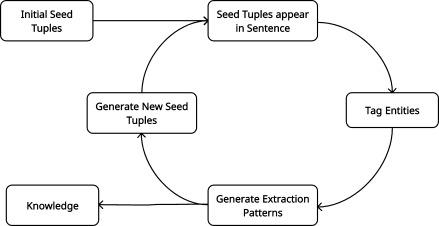
\includegraphics
    [width=0.8\textwidth]{image/parts/4}
    \begin{center}
        \begin{tablenotes}
        \end{tablenotes}
    \end{center}
    \renewcommand{\figurename}{Hình.}
    \caption{Phương pháp học bán giám sát (Semi-Supervised Learning) để trích xuất quan hệ.}\label{fig:figure3}
\end{figure}

\newpage
\subsubsection{Phương pháp giám sát từ xa (Distant supervision)}
Phương pháp này còn được gọi là phương pháp giám sát yếu (weakly supervised methods) hoặc phương pháp dựa trên
kiến thức (knowledge based methods).
\href{https://www.sciencedirect.com/science/article/pii/S2667305323000698#br0890}{Mintz et al. (2009)}
đã đề xuất phương pháp giám sát từ xa, trong đó dữ liệu huấn luyện được tạo tự động bằng cách liên kết văn bản với một
Cơ sở tri thức (Knowledge Base - KB). Điều này giúp loại bỏ vấn đề dán nhãn thủ công cho dữ liệu huấn luyện. Học từ xa
dựa trên giả định rằng nếu hai thực thể có quan hệ xuất hiện trong KB, thì tất cả các cụm từ đề cập đến hai thực thể này
đều có thể diễn đạt mối quan hệ đó.

\begin{singlespace}
Theo cách này, Giám sát từ xa sử dụng cơ sở tri thức, chẳng hạn như Freebase, để trích xuất các mối quan hệ giữa hai đối
tượng.
Khi cùng một cặp thực thể xuất hiện trong cả một câu và một KB, thì theo quy tắc heuristic, câu đó được liên kết
với mối quan hệ khớp từ KB. Ví dụ, hãy xem xét câu: \('\)Bill Gates là người sáng lập Microsoft.\('\) Nếu người \('\)Bill Gates\('\) và
tổ chức \('\)Microsoft\('\) xuất hiện dưới dạng bộ ba \('\)(entity1: Bill Gates, entity2: Microsoft, relation: founder_of)\('\) trong Freebase,
thì hai thực thể này đại diện cho mối quan hệ founder\_of (người sáng lập).
Smirnova và Cudré-Mauroux (2018) đã sử dụng một
quy trình như được thể hiện trong \href{https://www.sciencedirect.com/science/article/pii/S2667305323000698#fg0040}{Hình 4}
để tạo dữ liệu huấn luyện bằng Giám sát từ xa.
Các cách tiếp cận khác
(\href{https://www.sciencedirect.com/science/article/pii/S2667305323000698#br1150}{Riedel et al. (2010)}, \href{https://www.sciencedirect.com/science/article/pii/S2667305323000698#br1360}{Takamatsu et al. (2012)}, \href{https://www.sciencedirect.com/science/article/pii/S2667305323000698#br1540}{Zeng et al. (2014)}, \href{https://www.sciencedirect.com/science/article/pii/S2667305323000698#br1080}{Qin et al. (2018)}, \href{https://www.sciencedirect.com/science/article/pii/S2667305323000698#br0220}{Chen and Manning (2014)}, \href{https://www.sciencedirect.com/science/article/pii/S2667305323000698#br1110}{Quirk and Poon (2017)})
sử dụng Giám sát từ xa để trích xuất các mối quan hệ từ văn bản.
\end{singlespace}
